\newpage
\begin{question}
Represent the below graph with an adjacency matrix.

\begin{figure}[htb!]
  \centering
  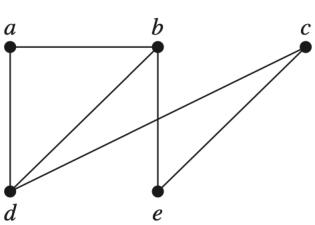
\includegraphics[width=0.3\linewidth]{q2_figure.pdf}
\end{figure}

\end{question}

\par\noindent\rule{\textwidth}{0.5pt}

\subsubsection*{Solutions}

The adjacency matrix for the graph is as follows:
\bigskip
\begin{center}
\begin{tabular}{|c|ccccc|}
  \hline
  & a & b & c & d & e \\
  \hline
  a & 0 & 1 & 0 & 1 & 0 \\
  b & 1 & 0 & 0 & 1 & 1 \\
  c & 0 & 0 & 0 & 1 & 1 \\
  d & 1 & 1 & 1 & 0 & 0 \\
  e & 0 & 1 & 1 & 0 & 0 \\
  \hline
\end{tabular}
\end{center}
,
$$
\begin{bmatrix}
  0 & 1 & 0 & 1 & 0 \\
  1 & 0 & 0 & 1 & 1 \\
  0 & 0 & 0 & 1 & 1 \\
  1 & 1 & 1 & 0 & 0 \\
  0 & 1 & 1 & 0 & 0 \\
\end{bmatrix}
$$
